\section*{Image Examples of Results}

A selection of images from the Vienna City Poster Dataset is presented, with predictions and ground truth bounding boxes and labels. Red colour is for predictions and green for ground truth. Also I added comments on used method and achieved CER score. Some images are cropped because in the upper part of the picture is no text and results are then better comparable. First I have chosen images with good results and well legible text, then I have chosen images with complicated text for detection and recognition. They are readable by a human but machines might struggle because they remind more of images than letters, or are only half visible and strong contextual information is needed. 


%--------balerina image
\subsection*{P-117050}
This image has well readable letters and for all tested models this image was not difficult to read and only minor mistakes occurred.

\begin{figure}[hbtp!]
    \centering
    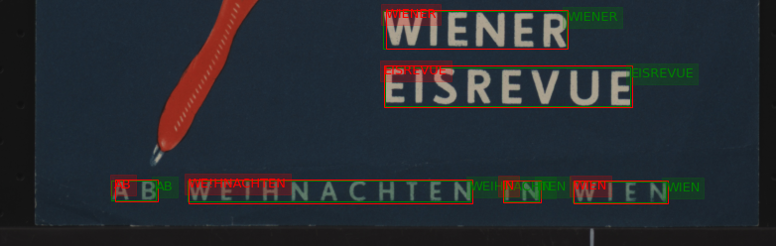
\includegraphics[scale=0.36]{obrazky/plakaty/result_easyOCR_vienna1_split_tuning_special_sensitive-21.png}
    \caption{EasyOCR, tuning}
    \label{Im2:ex:easy}
\end{figure}

\begin{figure}[hbtp!]
    \centering
    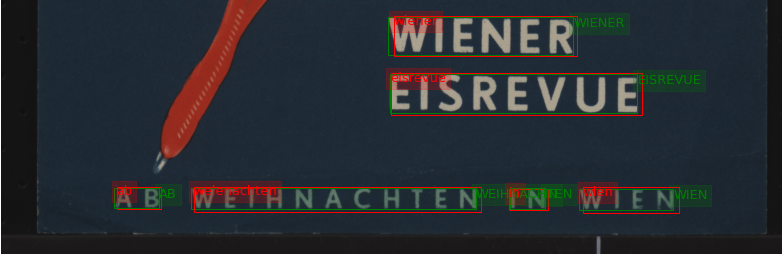
\includegraphics[scale=0.36]{obrazky/plakaty/result_kerasOCR_vienna1_nosplit_nocorrection-21.png}
    \caption{Keras-OCR, untrained}
    \label{Im2:ex:keras}
\end{figure}

\begin{figure}[hbtp!]
    \centering
    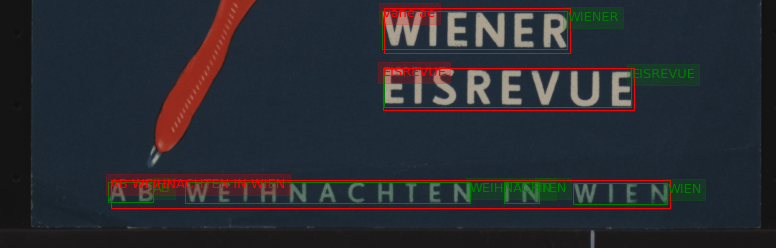
\includegraphics[scale=0.36]{obrazky/plakaty/result_carfttesseract_vienna1_split-21.png}
    \caption{Tesseract+CRAFT}
    \label{Im2:ex:Craft}
\end{figure}

\begin{figure}[hbtp!]
    \begin{subfigure}{\textwidth}
        \centering
        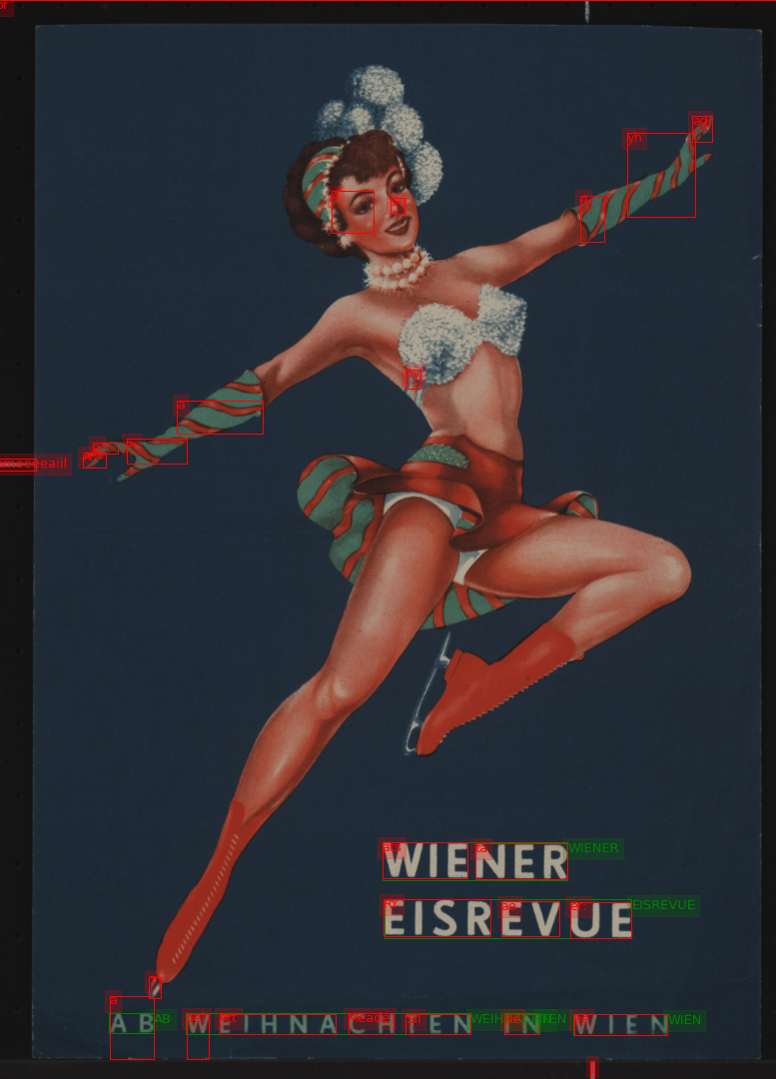
\includegraphics[scale=0.36]{obrazky/plakaty/result_tesseract_vienna1_nosplit_psm11-21.png}
        \caption{PSM 11}
        \label{Im2:ex:tess11}
    \end{subfigure}

    \begin{subfigure}{\textwidth}
        \centering
        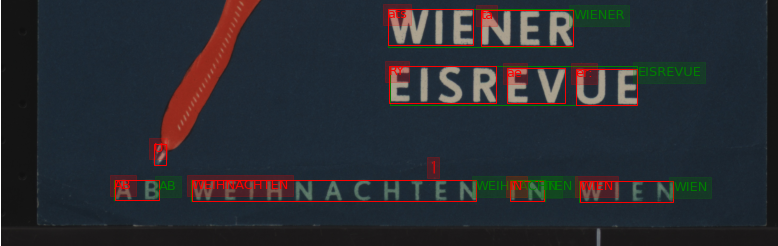
\includegraphics[scale=0.36]{obrazky/plakaty/result_tesseract_vienna1_split_psm4-21.png}
        \caption{PSM 4}
        \label{Im2:ex:tess4}
    \end{subfigure}
    \caption{Tesseract}
    \label{Im2:ex:tess}
\end{figure}


\subsection*{P-2638}

\begin{figure}[hbtp!]
    \begin{subfigure}{\textwidth}
        \centering
        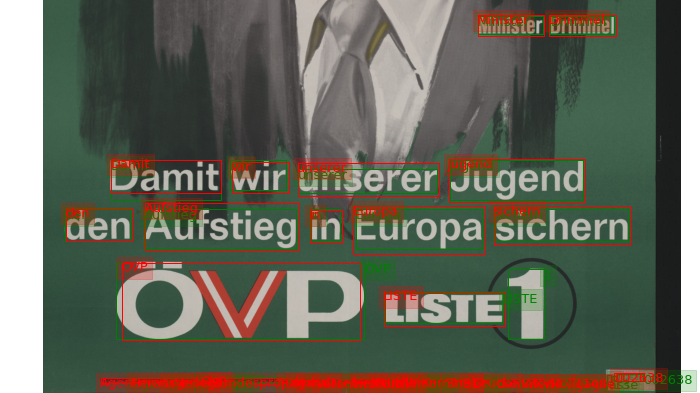
\includegraphics[scale=0.36]{obrazky/plakaty/result_easyOCR_vienna1_split_tuning-91.png}
        \caption{tuning}
        \label{Im1:ex:easytun}
    \end{subfigure}

    \begin{subfigure}{\textwidth}
        \centering
        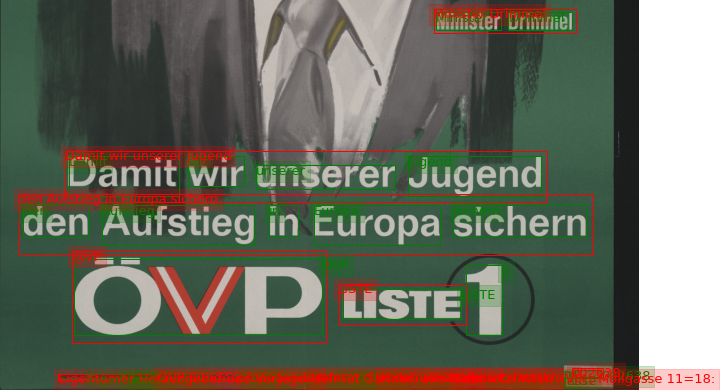
\includegraphics[scale=0.36]{obrazky/plakaty/result_easyOCR_vienna1_nosplit_notuning-91.png}
        \caption{no tuning}
        \label{Im1:ex:easy}
    \end{subfigure}
    \caption{EasyOCR}
    \label{Im1:ex:EasyOCR}
\end{figure}

\begin{figure}[hbtp!]
    \begin{subfigure}{\textwidth}
        \centering
        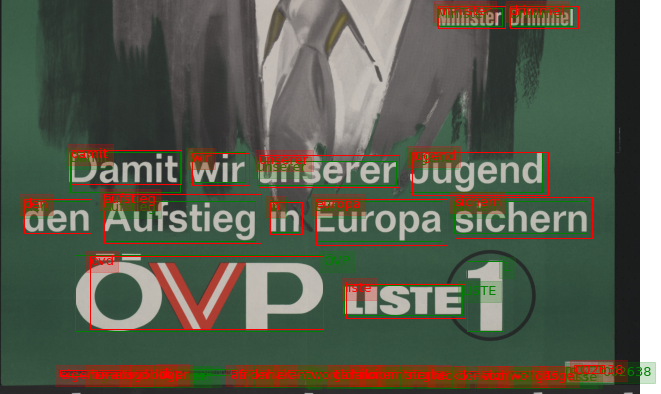
\includegraphics[scale=0.36]{obrazky/plakaty/result_kerasOCRtrained_vienna1_split-90.png}
        \caption{Keras-OCR, trained}
        \label{Im1:ex:kertr}
    \end{subfigure}

    \begin{subfigure}{\textwidth}
        \centering
        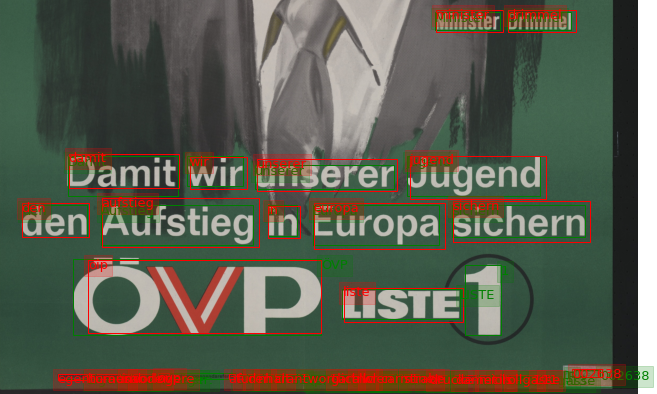
\includegraphics[scale=0.36]{obrazky/plakaty/result_kerasOCR_vienna1_nosplit_nocorrection-90.png}
        \caption{Keras-OCR}
        \label{Im1:ex:ker}
    \end{subfigure}
    
    \caption{Keras-OCR}
    \label{Im1:ex:Keras}
\end{figure}


\begin{figure}[hbtp!]
    \centering
    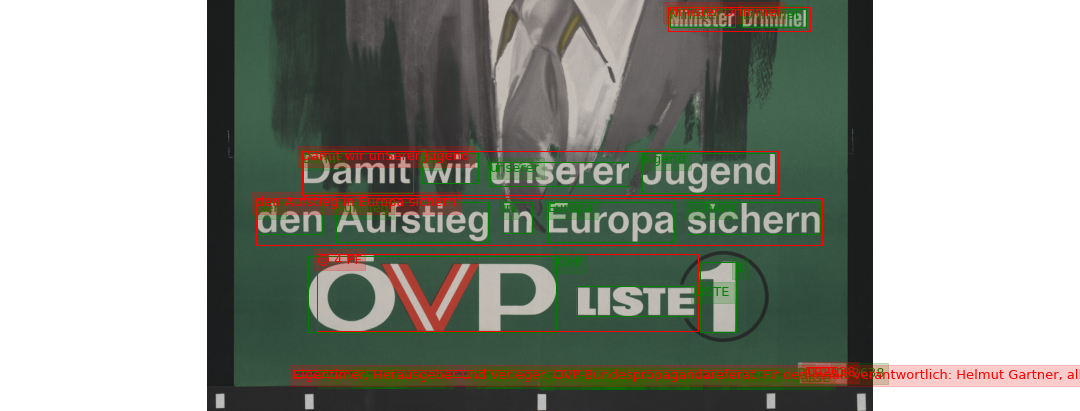
\includegraphics[scale=0.36]{obrazky/plakaty/result_carfttesseract_vienna1_split_special_snesitive-91.png}
    \caption{Tesseract+CRAFT}
    \label{Im1:ex:craft}
\end{figure}


\begin{figure}[hbtp!]  
      \centering
    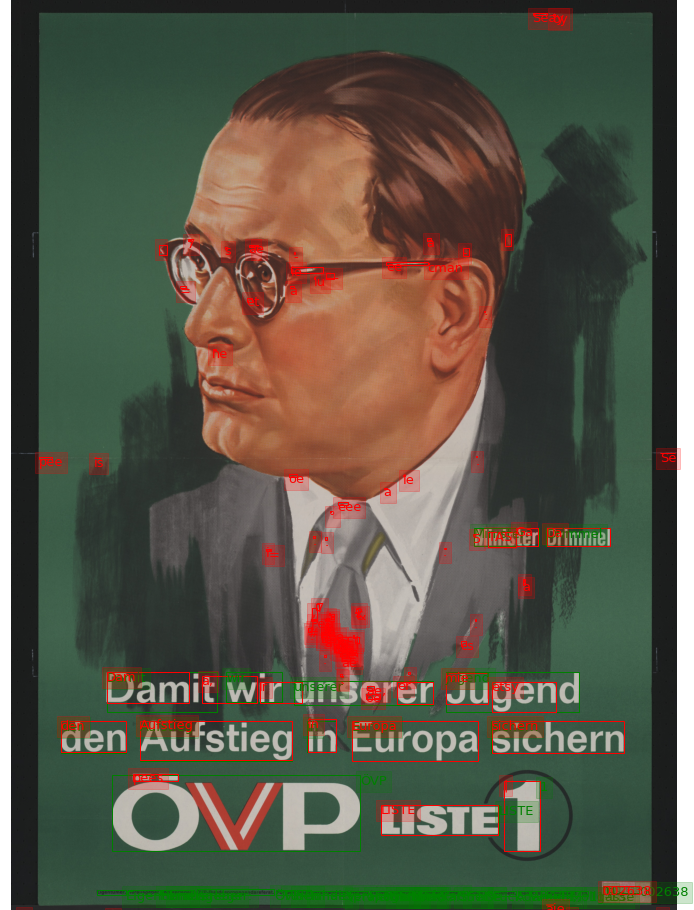
\includegraphics[scale=0.36]{obrazky/plakaty/result_tesseract_vienna1_split_psm11-91.png}
    \caption{Tesseract, PSM 11. Tesseract found many non existing words and tried to predict them.}
    \label{Im1:ex:tess11}
\end{figure}

\subsection*{P-315617}

\begin{figure}[hbtp!]
    \begin{subfigure}{\textwidth}
        \centering
        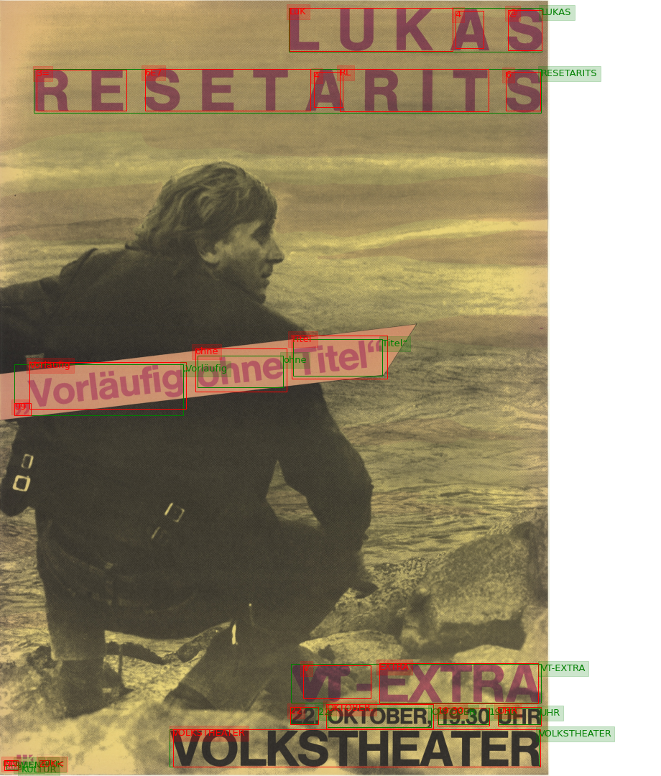
\includegraphics[scale=0.29]{obrazky/plakaty/result_easyOCR_vienna2_nosplit_tuning-83.png}
        \caption{tuning}
        \label{Im3:ex:easytun}
    \end{subfigure}

    \begin{subfigure}{\textwidth}
        \centering
        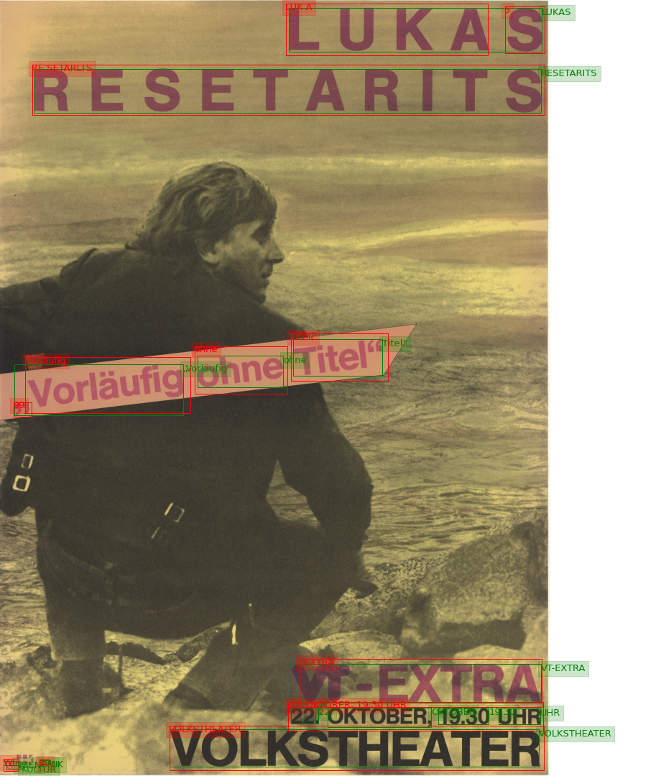
\includegraphics[scale=0.29]{obrazky/plakaty/result_easyOCR_vienna2_nosplit_notuning_nocorrection-83.png}
        \caption{no tuning}
        \label{Im3:ex:easy}
    \end{subfigure}
    \caption{EasyOCR}
    \label{Im3:ex:EasyOCR}
\end{figure}

\begin{figure}[hbtp!]
    \centering
   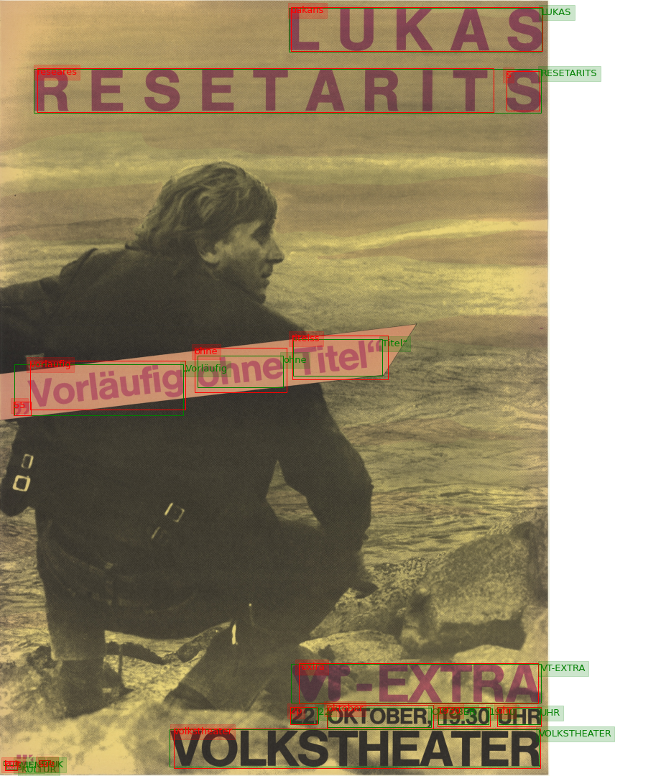
\includegraphics[scale=0.3]{obrazky/plakaty/result_kerasOCR_vienna2_nosplit-83.png}
    \caption{Keras-OCR, untrained}
    \label{Im3:ex:keras}
\end{figure}

\begin{figure}[hbtp!]
    \centering
    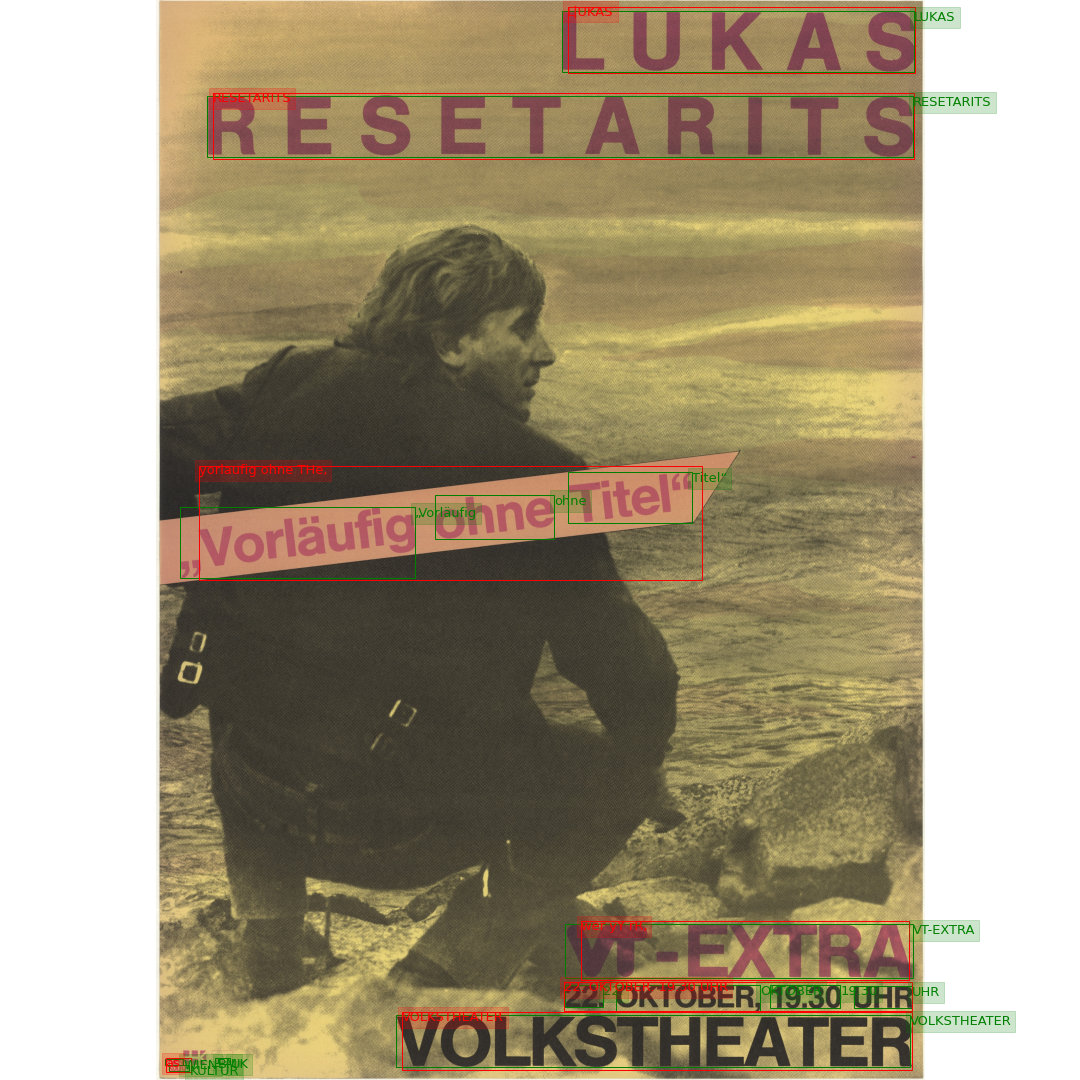
\includegraphics[scale=0.3]{obrazky/plakaty/result_carfttesseract_vienna2_split_special_snesitive-83.png}
    \caption{Tesseract+CRAFT}
    \label{Im3:ex:craft}
\end{figure}

\begin{figure}[hbtp!]
    \begin{subfigure}{0.45\textwidth}
        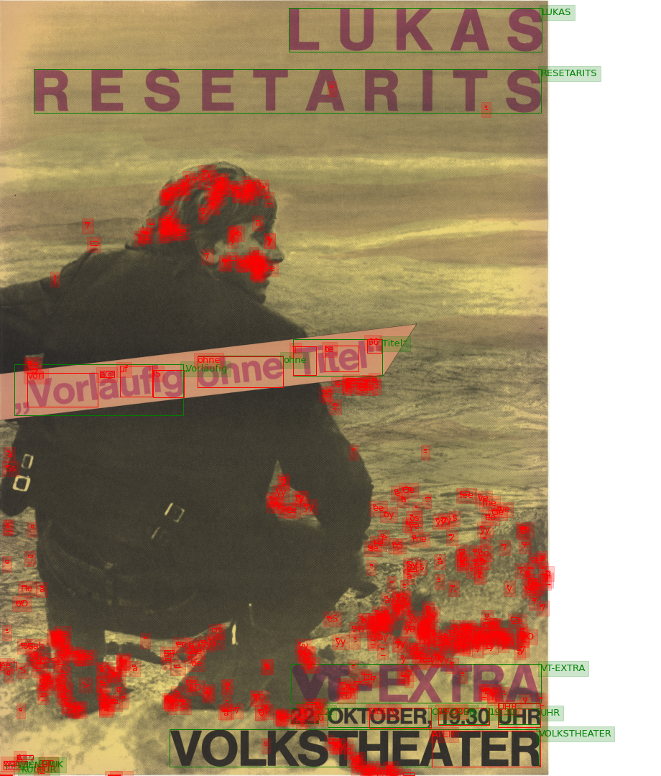
\includegraphics[scale=0.29]{obrazky/plakaty/result_tesseract_vienna2_nosplit_psm11-83.png}
        \caption{PSM 11. Tesseract found many non existing words and tried to predict them.}
        \label{Im4:ex:tess11}
    \end{subfigure}

    \begin{subfigure}{0.45\textwidth}
        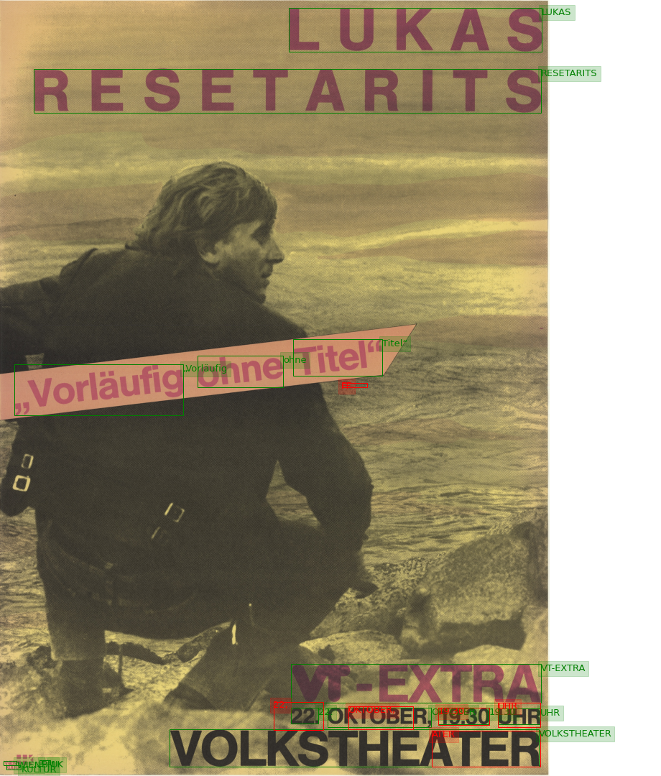
\includegraphics[scale=0.29]{obrazky/plakaty/result_tesseract_vienna2_split_psm4-83.png}
        \caption{PSM 4}
        \label{Im4:ex:tess4}
    \end{subfigure}

    \caption{Tesseract}
    \label{Im3:ex:tess}
\end{figure}

\subsection*{P-236873}
% result_easyOCR_vienna1_split_tuning_special_sensitive-55.png
% result_easyOCR_vienna2_nosplit_notuning_nocorrection-70.png

This image has a text that is supposed to look like northern lights in a night sky and is not easy to read even by humans. None of the models were able to identify the wavy text.

\begin{figure}[hbtp!]
    \begin{subfigure}{0.5\textwidth}
        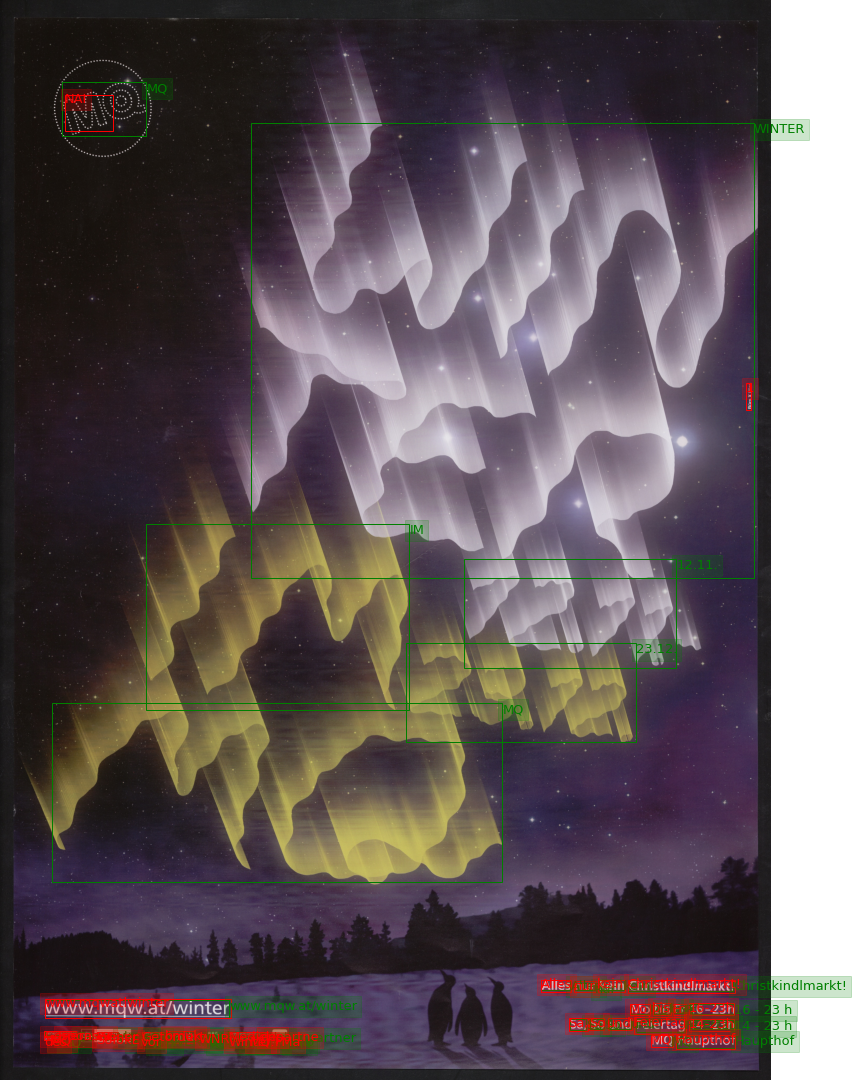
\includegraphics[scale=0.3]{obrazky/plakaty/result_easyOCR_vienna1_split_tuning_special_sensitive-73complecatedP-236873.png}
        \caption{EasyOCR}
        \label{Im4:ex:easy}
    \end{subfigure}
    \begin{subfigure}{0.45\textwidth}
        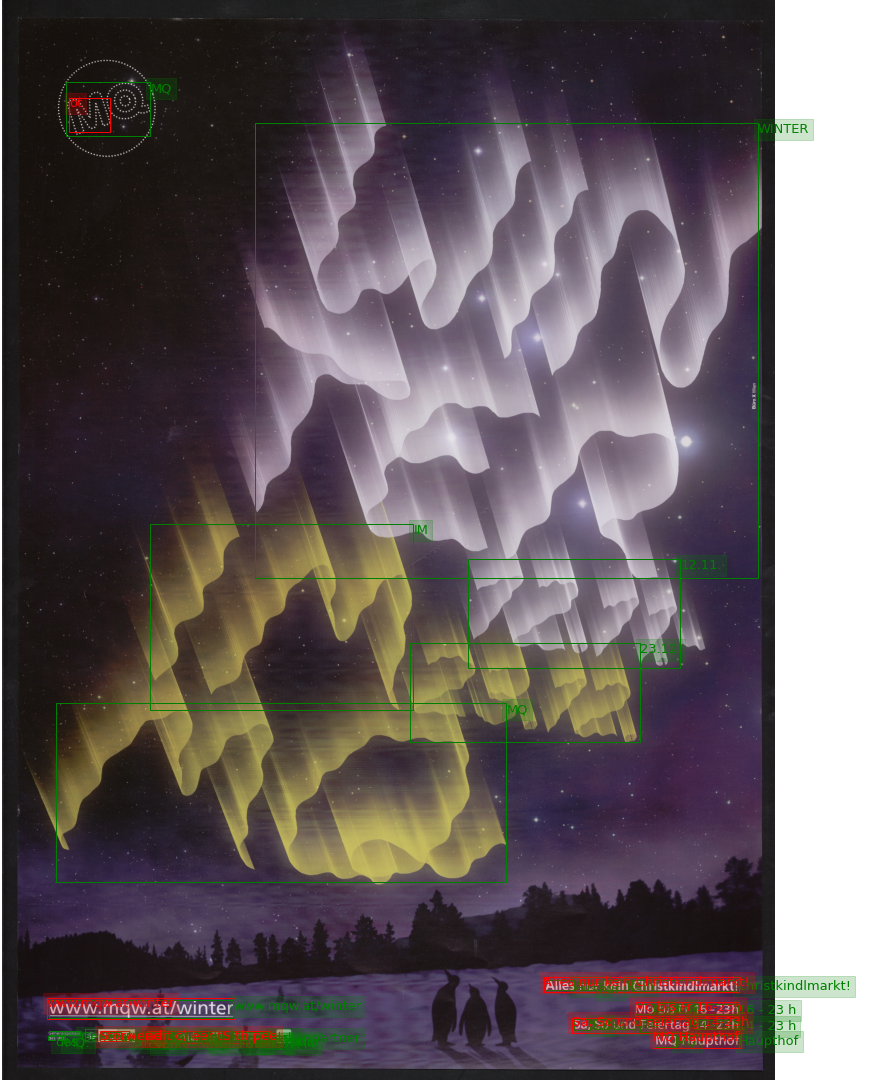
\includegraphics[scale=0.3]{obrazky/plakaty/result_carfttesseract_vienna1_split_special_snesitive-73.png}
        \caption{Tesseract+CRAFT}
        \label{Im4:ex:craft}
    \end{subfigure}

    \caption{Tesseract}
    \label{Im4:ex:compl}
\end{figure}

\subsection*{P-229767}
This image is a challenge for the detector and recognizer because there is a large number 10. The height and width of the number is same as the dimensions of the whole image and on top of that the number zero is not completely visible. Then there is curved text, which is also challenging. 

\begin{figure}[hbtp!]
    \centering
    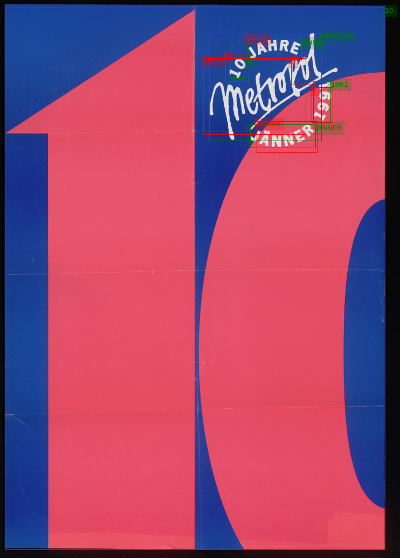
\includegraphics[scale=0.8]{obrazky/plakaty/result_easyOCR_vienna1_split_tuning_special_sensitive-55.png}
    \caption{EasyOCR on image P-}
    \label{Im5:ex:easy}
\end{figure}

\subsection*{P-310877}
This image has a very spexific font, which without former knowledge is very difficult to recognize.

\begin{figure}[hbtp!]
    \centering
    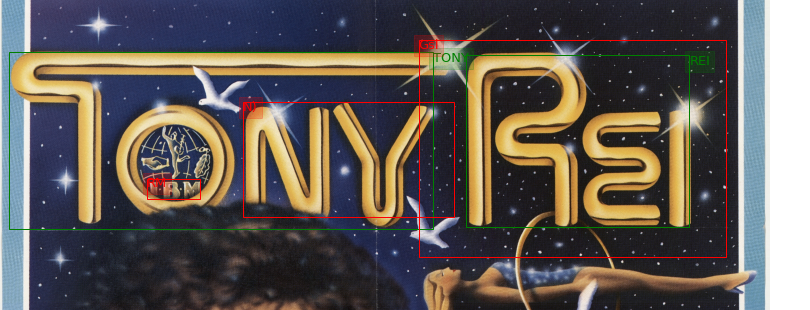
\includegraphics[width=\textwidth]{obrazky/plakaty/result_easyOCR_vienna2_nosplit_notuning_nocorrection-70.png}
    \caption{EasyOCR on image P-}
    \label{Im6:ex:easy}
\end{figure}


\subsection*{P-231248}
This image demonstrates that vertical text is more complicated for the recognizer although it is quite legible.

\begin{figure}[hbtp!]
    \centering
    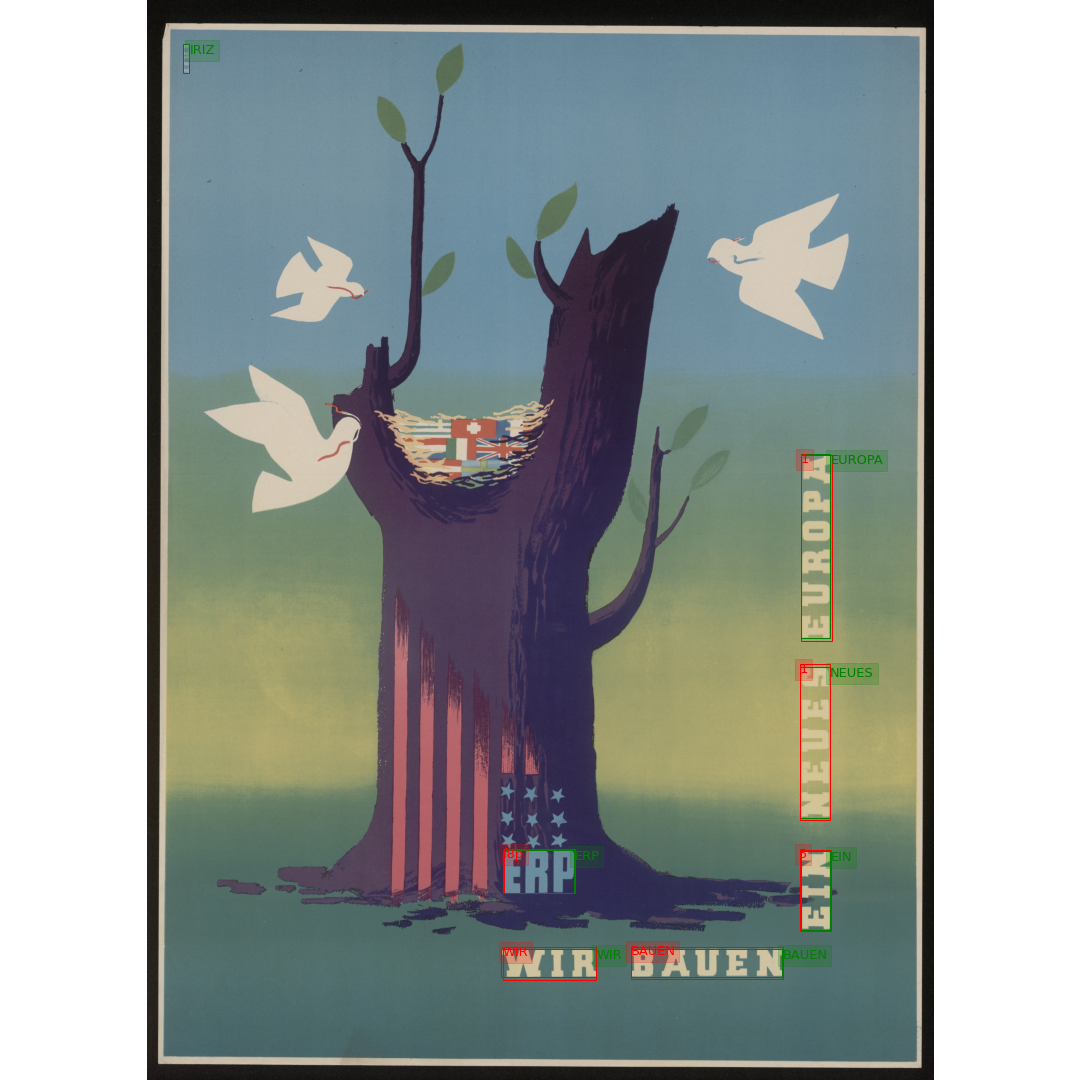
\includegraphics[width=\textwidth]{obrazky/plakaty/result_easyOCR_vienna1_split_tuning_special_sensitive-60verticaltextproblem.png}
    \caption{EasyOCR on image P-}
    \label{Im7:ex:easy}
\end{figure}




